%%%%%%%%%%%%%%%%%%%%%%%%%%%%%PREÁMBULO DEL DOCUMENTO%%%%%%%%%%%%%%%%%%%%%%%%%%%
% En esta sección se configura el documento, pero no se incluye contenido

% Esto es la clase del documento, que define las instrucciones principales
% que condicionarán el documento generado. Generalmente cambiarla después de 
% añadir contenido produce numerosos errores.
\documentclass[]{article}


%%%%%%%%%%%%%%%%%%%SECCIÓN INCLUSIÓN DE PAQUETES %%%%%%%%%%%%%%%%%%%%%%%%%%%%%%
% Este paquete permite cambiar la fuente. Hay muchas, la lista se puede
% encontrar en https://tug.org/FontCatalogue/, las que no indican nada después
% del nombre son las que se pueden usar como está aquí puesto.
\usepackage[T1]{fontenc}
% Comentar esta línea haría que se usara la fuente predeterminada.
%\usepackage{newcent}
\usepackage{titlesec}

% Carga el paquete babel, las opciones son:
    % spanish: indica que usaremos configuración para escribir en español
    % es-tabla: traduce la palabra table como tabla, no como cuadro
    % es-lcroman: permite la numeración romana en minúscula.
\usepackage[spanish,es-tabla]{babel}
% Paquete que permite escribir el símbolo del euro, se usa de dos maneras.
    % En el documento, la orden \euro escribirá el símbolo
    % Si se escribe \EUR{<cifra>} el paquete formará un bloque con el
    % número y el símbolo.
    % El símbolo del euro que pone es el «oficial» es decir, no se adapta
    % a la fuente que se use.
\usepackage{eurosym} 
% Paquete para que las imágenes tengan un tamaño relativo al del párrafo
\usepackage{graphicx}
% nos permite insertar las figuras con el especificador H, que hace que se
    % inserte en el lugar del document donde se ha escrito su código.
\usepackage{float} 
% Paquete que habilita las referencias cruzadas.
\usepackage{hyperref}
% Permite poner pies y encabezados de página personalizados
\usepackage{fancyhdr}
 %permite referenciar la última página (para incluir páginas totales)
\usepackage{lastpage}
% Paquete BibTex para referencias bibliográficas.
\usepackage[backend=biber, style=apa, citestyle=apa]{biblatex}
% Añadimos un archivo de fuentes bibliográficas.
\addbibresource{bibliography/sources.bib}
% Paquete para cambiar la configuración de página.
\usepackage{geometry}
%Cambiamos los márgenes de página
\geometry{
    a4paper, % tamaño del papel
    left=30mm, % márgenes laterales
%   top=50mm 
    bottom=35mm, %margen inferior
    headheight=25mm    %margen superior
}

% Permite el uso de más caracteres, aunque algunos especiales siguen sin
% estar disponibles.
\usepackage[utf8]{inputenc}

%Permite utilizar la fuente de trazo doble en ecuaciones.
\usepackage{amsfonts}
%%%%%%%%%%%%%%%%%%%% FIN SECCIÓN %%%%%%%%%%%%%%%%%%%%%%%%%%%%%%%%%%%%%%%%%%%%%%

% Vamos a permitir más niveles de título, hasta 5.
\setcounter{secnumdepth}{5}
% Esto hace que la tabla de contenidos muestre hasta el nivel 3.
    % Si se quiere que la tabla de contenido muestre todos los niveles, sólo
    % ha de cambiarse el 3 por un 5
\setcounter{tocdepth}{3}
% Aquí estamos redefiniendo el comando paragraph, será nuestro título de nivel
    % 4. Esta es una de las cosas que no tengo nada claro cómo funciona, 
    % pero funciona, así que si quieres usar títulos de esta jerarquía, 
    % déjalo así. 
\titleformat{\paragraph}{\bfseries}{\theparagraph .}{1em}{}
\titlespacing*{\paragraph}{0pt}{3.25ex plus 1ex minus .2ex}{1.5ex plus .2ex}

% El subparagraph será el título de nivel 5
\titleformat{\subparagraph}{\bf}{\thesubparagraph .}{1em}{}
\titlespacing*{\subparagraph}{0pt}{3.25ex plus 1ex minus .2ex}{1.5ex plus .2ex}


% Esta línea nos permite indicar un directorio donde estamos guardando
% nuestras imágenes. Más información más adelante.
\graphicspath{{img/}}


% Esto hace que los enlaces a webs (\href{url}{texto} salgan en azul.
    % También impide que salga un repugnante cuadrado rojo alrededor de cada
    % referencia cruzada que incluyas en el documento.
\hypersetup{
    colorlinks=true,
    linkcolor=black,
    filecolor=magenta,      
    urlcolor=blue,
    citecolor=black
}

% Permite que en las ecuaciones escribas un punto y salga un punto (no lo
% interprete como un decimal en español, es decir, una coma)
\decimalpoint


%%%%%%%%%%%%%%%%%SECCIÓN VARIABLES %%%%%%%%%%%%%%%%%%%%%%%%%%%%%%%%%%%%%%%%%%%%
% Podemos definir variables para usar a lo largo del texto
% Así podemos cambiarlas aquí sin tener que repetir texto.
\def \autor{Francisco Rodríguez Melgar}
\def \titulo{Ejemplo de documento en \LaTeX{}}
\def \organizacion{Universidad de Ejemplo}
%%%%%%%%%FIN SECCIÓN%%%%%%%%%%%%%%%%%%%%%%%%%%%%%%%%%%%%%%%%%%%%%%%%%%%%%%%%%%%

% Esta orden especifica que cuando se cree la portada se use este título.
% Además, con Huge utilizamos la macro de tipo de letra más grande que hay 
% disponible.
\title{\textbf{\Huge{\titulo}}}
% Aquí lo mismo, pero con el autor
% Algunos especificadores de tamaño son: tiny, small, large, Large, LARGE, huge
    % y Huge
\author{\LARGE{\autor}\\ \\ \Large{\organizacion}}
%%%%%%%%%%%%%%%%%%%%%%%%%%%%FIN DEL PREÁMBULO%%%%%%%%%%%%%%%%%%%%%%%%%%%%%%%%%%


%%%%%%%%%%%%%%%%%%%%%%%%%%%%%%INICIO DEL DOCUMENTO%%%%%%%%%%%%%%%%%%%%%%%%%%%%%
% La totalidad del texto que se renderizará en PDF en tu documento debe estar
% entre begin document y end document.
\begin{document}
% Elimina la numeración de página hasta que se diga lo contrario.
\pagenumbering{gobble}
% Pone el título, el autor y la fecha. (la fecha se detecta automáticamente)
\maketitle

% Aquí creamos una figura para poner el logo de algo (Ahora hay un placeholder) 
% más en cuanto a figuras más adelante.
\begin{figure}[H]
    % Lo centramos
    \center
    
\includegraphics[width=.5\linewidth]{escudo}
\end{figure}
\newpage

% En esta página puedes poner agradecimientos o prefacios que no tendrán pie ni
% encabezado de página y que no afectarán a la numeración, si no quieres poner
% nada, elimina esta línea y uno de los newpages
\begin{center}
\textbf{[Esta página ha sido dejada en blanco a propósito por el editor]}
\end{center}
\newpage
%Vamos a poner agradecimientos. El bloque flushright alinea el texto a la 
    % derecha.
\begin{flushright}
\textit{Esto es un placeholder, muchas gracias, placeholder.}
\end{flushright}
\newpage % salto de página

%%%%%%%%%%%%%%%%% CABECERA Y PIE DE PÁGINA SECCIÓN ÍNDICE%%%%%%%%%%%%%%%%%%%%%
\pagestyle{fancy}
\fancyhf{}
\fancyhead[C]{
\Large\titulo\normalsize\\
\rule[1mm]{0.3\hsize}{.5pt}\\
ÍNDICES
}
% Incluye el texto "pág. X de Y" en el pie de pág. a la derecha.
    % estoy referenciando una etiqueta que añadí, se verá luego.
\rfoot{pág. \textsc{\thepage{}} de \textsc{\pageref{startSectionContent}}} 
% Incluye una línea en el pie de página.
\renewcommand{\footrulewidth}{0.5pt}
%decimos que se numeren las páginas en romano hasta nueva orden
    % Esto nos permite numerar las páginas de índices en números romanos
\pagenumbering{roman} 
%%%%%%%%%%%%%%%%%                 FIN                      %%%%%%%%%%%%%%%%%%%
\tableofcontents %crea el índice el índice empieza siempre en página nueva

% se pueden añadir saltos de página extra con \newpage
\newpage

% cambia el nombre del índice de ilustraciones
%\renewcommand{\listfigurename}{Índice de ilustraciones}
%inserta el índice de ilustraciones
\listoffigures 
\newpage

%cambia el nombre del índice de tablas
%\renewcommand{\listtablename}{Índice de tablas}
%inserta el índice de tablas
\listoftables

% Esta orden (label) inserta etiquetas invisibles en el texto, al ponerla justo
    % antes del salto de página del último índice de la sección, me permite
    % referenciar este punto, así es como consigo que salga "Pág. i de iii".
\label{startSectionContent}
\newpage
% A partir de aquí numeración normal
\pagenumbering{arabic}
%%%%%%%%%%%%%%%%% CABECERA Y PIE DE PÁGINA SECCIÓN CUERPO%%%%%%%%%%%%%%%%%%%%%%
\pagestyle{fancy}
\fancyhf{}
\fancyhead[C]{
\Large\titulo\normalsize\\
\rule[1mm]{0.3\hsize}{.5pt}\\
\leftmark
}
% El único cambio es que aquí referencio la última página del documento.
\fancyfoot[R]{pág. \thepage{} de \pageref{LastPage}}
\fancyfoot[L]{\today}
\renewcommand{\footrulewidth}{0.5pt}
%%%%%%%%%%%%%%%%%%%%%%%%%%%%%%%%%FIN SECCIÓN%%%%%%%%%%%%%%%%%%%%%%%%%%%%%%%%%%%
% La sección es el primer nivel de título que se permite en esta clase de 
    % documento. Introduce un título de primer nivel
\section{Presentación}
Este documento pretende ser un ejemplo de varias tareas que se suelen realizar
en LaTeX. Se recomienda compilar el código y ver el pdf y el código a la
vez para ver los resultados. En los comentarios del código explico lo que se va
haciendo y qué órdenes son necesarias para crear lo que se ve en el PDF.
Además, incluyo un \textit{script} de compilación mínimo que debería compilar
sin problemas. Los prerrequisitos para utilizar la compilación automática son:

\begin{itemize}
    \item Sistema UNIX like (GNU/Linux o Mac OS).
    \item Editor de ficheros de texto plano en el equipo (notepad, Notepad++,
        Sublime, Vim, Nano...)
    \item Programa pdflatex instalado en el equipo
    \item Utilidad make instalada en el equipo.
\end{itemize}

En caso de tener un sistema operativo Windows, deben seguirse las instrucciones
de instalación que se detallan en la siguiente sección.
\subsection{Instalación}
La instalación de \LaTeX{} es sencilla tanto en sistemas operativos GNU/Linux
como en sistemas operativos Windows.
\subsubsection{Instalación en GNU/Linux}\label{instGNULinux}
En la mayoría de instalaciones de escritorio de Linux se incluye un editor de
texto plano, ya sea éste Nano, Emacs, Vim u otros. Esos editores son válidos para
crear (o abrir) archivos \texttt{.tex}. Para instalar \LaTeX{} se puede hacer
en la mayoría de distribuciones mediante el gestor de paquetes, por ejemplo, en
las distribuciones derivadas de Debian (Ubuntu, Kubuntu, Xubuntu, Linux Mint...)
se puede instalar con la siguiente orden:
\begin{verbatim}
sudo apt install texlive-base \
texlive-latex-recommended \
texlive-latex-extra \
texlive-full
\end{verbatim} 
En otras distribuciones, 
por favor, consulte la documentación específica de cómo instalar paquetes de
\textit{software}.

Una vez instalados estos paquetes, se puede compilar con el comando
\texttt{pdflatex}, este comando debería ejecutarse sobre un archivo .tex.
(ver \textbf{\ref{ArchivosTex}}).

Una vez instalado todo esto, en sistemas Linux se puede compilar este 
documento con el comando \texttt{make}. Para ello debe instalarle si no se
tiene ya instalado. Para hacerlo, de nuevo, en distribuciones derivadas de
Debian con este comando:
\begin{verbatim}
sudo apt install make
\end{verbatim}

Si quieres preparar un entorno para compilar archivos (en Linux) que hayas
escrito tú, simplemente crea un directorio en sitio sencillo (por ejemplo tu
carpeta personal) y, dentro del mismo, un archivo .tex. Por ejemplo, con estos
comandos de terminal se puede hacer:
\begin{verbatim}
mkdir ~/holaMundoLatex
touch ~/holaMundoLatex/holaMundo.tex
cd ~/holaMundoLatex
\end{verbatim}

Con estos comandos habrás creado un directorio en tu carpeta personal llamado
\texttt{holaMundoLatex}, un documento .tex dentro llamado \texttt{holaMundo.tex}
y te habrás situado en él para trabajar. En las páginas siguientes podrás ver
cómo crear el primer documento. Recuerda que el fichero de este tutorial dispone
de compilación con \texttt{make}, los que tú crees no.

\subsubsection{Instalación en Microsoft Windows}
En sistemas Windows, la instalación se realiza como otras herramientas de
\textit{software}, se descarga un \texttt{.exe} y se siguen las instrucciones
del instalador. En nuestro caso, debemos instalar dos programas:
\begin{itemize}
    \item MikTex, el <<motor>> de \LaTeX{}, que nos permitiría compilar,
         pero sin ofrecernos asistencia a la edición.
        Este programa se puede descargar desde
         \href{https://miktex.org/download}{aquí}. 
    \item TexStudio, el editor de documentos \LaTeX{}, que nos permite compilar
        sin tener que usar la línea de comandos de Windows. Y nos ofrece
        asistencia a la edición y funcionalidades como corrector ortográfico.
        Se puede descargar desde \href{https://www.texstudio.org/}{aquí}.
\end{itemize}

Durante el proceso de
instalación de MikTex se nos hará decidir la ruta de instalación y si permitimos
que el programa descargue de internet los paquetes necesarios. Yo
recomiendo permitirle hacerlo. Para ello se deben dejar las opciones como
se ve en la Figura \ref{fig:miktex}: \nameref{fig:miktex}.
\begin{figure}[H]
    \center
    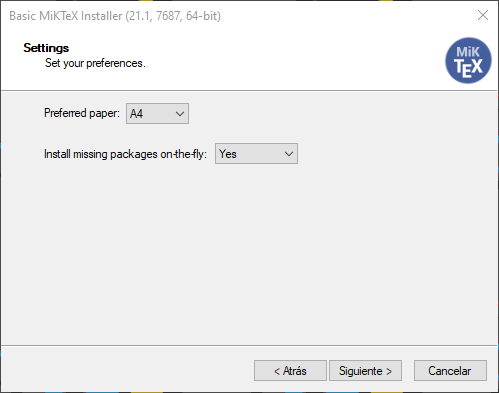
\includegraphics[width=0.75\hsize]{miktexInstall}
    \caption{Opciones de instalación de MikTex}
    \label{fig:miktex}
\end{figure}

Cuando se tengan los dos programas instalados, deberá abrirse el fichero
\texttt{document.tex} que se encuentra en esta carpeta
con el segundo programa (TexStudio). Una vez hecho hecho, debe pulsarse la tecla
F5, que nos compilará el documento, generará el pdf y mostrará el resultado a la
derecha como se puede ver en la figura \ref{fig:texstudio}:
\nameref{fig:texstudio}. Como este ejemplo incluye referencias bibliográficas,
no se van a crear bien, porque hacen falta pasos adicionales para eso, pero
se generará el PDF, y en secciones posteriores se explica lo que hay que hacer.

\begin{figure}[H]
    \center
    \includegraphics[width=1.0\hsize]{TexStudio}
    \caption{Ventana principal de TexStudio}
    \label{fig:texstudio}
\end{figure}

Este documento está diseñado para ser una guía básica sobre Latex, pero para
poder generarse, se usarán comandos en el mismo documento antes de explicarlos.
Si se sabe algo sobre \LaTeX{} es recomendable leer el código primero, si no, 
mejor leer primero el pdf compilado.

\newpage\section{Comandos básicos de \LaTeX{}}
Aunque en este documento no voy a hablar de las características históricas o de
lo que es el \textit{typesetting}. Sí voy a explicar someramente qué es
\LaTeX{}. \LaTeX{} es un lenguaje que nos permite crear documentos con formato a
través de archivos de texto plano, que no contienen en sí mismos información
sobre el formato, sino que utilizan secuencias especiales de caracteres para
indicar cómo ha de presentarse el contenido en un documento distinto.
\subsection{Archivos .tex} \label{ArchivosTex}
Un archivo .tex es donde escribimos el código \LaTeX{}, es decir, la sucesión
de contenido y comandos que generará un documento. El
programa que genera el documento (generalmente pdf) a partir del código LaTeX
se llama motor o renderizador. Hay varios, con diferencias técnicas. Esta guía
y los comandos que se listan están desarrollados para el motor
\texttt{pdflatex}.

\subsubsection{Estructura de un archivo .tex}
Un documento en latex mínimo tiene estas líneas:
\begin{verbatim}
\documentclass{<clase del documento>}
\begin{document}
Algún texto.
\end{document}
\end{verbatim}

Para empezar: las palabras que van precedidas de una barra inclinada inversa
se llaman <<comandos>>, y son órdenes que se le dan al renderizador de \LaTeX{},
es decir, no se imprimirán en nuestro pdf (o no literalmente).
Debido a que los comandos se incluyen
con ese caracter especial, si quisiéramos escribir una barra inversa en el 
documento, deberíamos usar el comando \texttt{\textbackslash textbackslash}, 
seguido de un espacio. Si no, \LaTeX{} interpretaría que la siguiente palabra
es un comando. Además, los comandos reciben argumentos, que van entre llaves.
Como las llaves son otro carácter especial usado por el lenguaje, para 
incluirlas en nuestro texto, éstas deben ir precedidas de una barra inclinada
inversa, es decir, son otro comando: \texttt{\textbackslash \{} produciría:
<<\{>> (sin las comillas).

La clase del documento será una palabra que definirá un estilo de documento
concreto que nos permita empezar a escribir sin tener que formatearlo todo
desde 0. Las más populares son: article, book y report; pero hay muchas más.
Si se quiere compilar el primer documento en LaTeX, se puede copiar ese código,
pero debe sustituirse \texttt{<clase del documento>} por \texttt{article}.
Este documento se ha escrito con la clase de documento article. Como las clases
de documento definen las instrucciones que se usarán después en el documento,
es muy difícil cambiarla una vez se han escrito y formateado una cuantas
páginas.

Todo lo que hay antes de la línea donde pone 
\texttt{\textbackslash begin\{document\}}, sin incluirla, se denomina el 
\textbf{preámbulo del documento}. Y lo que existe entre la línea
\texttt{\textbackslash begin\{document\}} y la línea
\texttt{\textbackslash end\{document\}} se considera el contenido del
documento. En el preámbulo se incluyen numerosas órdenes que afectarán a cómo
el documento se renderiza, una de las más importantes es la inclusión de
paquetes, esto se hace mediante la orden \texttt{\textbackslash usepackage}.
Estos paquetes permiten añadir muchas funcionalidades que son necesarias. De 
hecho, hoy en día cualquier documento moderno incluye muchos paquetes. Si
se observa el preámbulo de este documento, se verá que hay, de hecho, muchos.

\textbf{Nota sobre paquetes:} para realizar muchas de las tareas que se explican
aquí se han incluido paquetes, para saber qué paquete es necesario para cada
cosa, acuda a los comentarios del código.

Ahora que ya hemos visto el contenido mínimo de un archivo .tex, puedes abrir
aquél que creaste en el punto \ref{instGNULinux} y copiar los ejemplos
que estamos viendo en él, para compilarlo en Linux y crear un pdf, puedes
ejecutar (recuerda situarte en el directorio donde creaste el archivo):
\begin{verbatim}
pdflatex holaMundo.tex
\end{verbatim}
En Windows, puedes abrir el archivo .tex con TexStudio y compilarlo con F5.

Además, por su herencia o similitud con otros lenguages formales,
de programación y de marcado, \LaTeX{} tiene la posibilidad de incluir 
comentarios en el código. Esto es texto que el renderizador no lee. En \LaTeX{}
dichos comentarios se ponen con el signo de porcentaje <<\%>>. Cualquier
texto en un archivo \texttt{.tex} que vaya en la misma línea que un signo de
procentaje y después de él no se renderizará. \textbf{Esto incluye el salto
de lína del final}. De nuevo, si se quiere incluir un signo de porcentaje
en el texto, debemos incluir antes de él una barra inclinada inversa, es decir:
\texttt{\textbackslash{\%}} generaría el signo de porcentaje.
Veamos un ejemplo:
\begin{verbatim}
\documentclass{article}
\begin{document} % Aquí puedo escribir lo que quiera
Algún texto de un párrafo.
% Este exto no va a salir
% Este tampoco.
Otro texto de otro párrafo.
\end{document}
\end{verbatim}

Además de que no se van a renderizar los textos de los comentarios, estos
dos párrafos son uno, porque se eliminan las líneas enteras, así que habría
que poner una línea en blanco entre el último comentario y el segundo
párrafo.

Al ser los documentos de \texttt{.tex} documentos de texto plano, podríamos
incluir potencialmente los caracteres que quisiéramos, pero, sin paquetes 
adicionales (ver sección de inclusión de paquetes en el código de este
documento) no se pueden incluir algunos símbolos. Así que hay que tener cuidado
con los símbolos especiales que se usan, pueden renderizarse mal o no permitir
que el pdf se genere. Si se usan los símbolos del idioma español: tildes, la eñe
diéresis en la u y demás, no debería haber problemas. Ej.: áéíóú, ÁÉÍÓÚ, üÜ, ñÑ.

\subsection{Escritura de texto en \LaTeX{}}
Como se ha visto en la sección anterior, dentro del contenido del documento es
donde se puede incluir texto. Ahora bien, si has experimentado con este archivo 
\texttt{.tex}.
que has creado con el código anterior, quizás hayas notado que los saltos de
línea no se trasladan a párrafos distintos.
En Latex, un párrafo es una línea de texto o varias líneas consecutivas, que se
renderizan siempre en el mismo párrafo salvo que haya una línea en blanco entre
ellas. Por ejemplo, vamos a poner un punto y aparte. Es decir:
\begin{verbatim}
\documentclass{article}
\begin{document}
Algún texto de un párrafo.

Otro texto de otro párrafo.
\end{document}
\end{verbatim}

Además, \LaTeX{} permite utlizar varios
comandos para manipular la presentación del texto.
\begin{itemize}
    \item \textbf{emph:} Pone el texto en énfasis.
    \item \textbf{textit:} Pone el texto en itálica (o cursiva).
    \item \textbf{textbf:} Pone el texto en negrita. 
    \item \textbf{texttt:} Utiliza fuente monoespaciada (como la de las máquinas
        de escribir).
    \item \textbf{textsc:} Pone el texto en versalitas (letras del mismo tamaño
    que las minúsculas, pero que se escriben como mayúsculas).
\end{itemize}
Estos comandos deben ponerse en nuestros archivos \texttt{.tex}
con una barra inclinada hacia atrás delante, como todos los comandos de 
\LaTeX{} y seguidos de dos llaves,
dentro de las cuales incluiremos el texto que queramos modificar. Por ejemplo:
\begin{verbatim}
Este es el primer párrafo de esta sección,
en cualquier texto podemos incluir texto en
\textbf{negrita} o en \textit{cursiva}, incluso,
podríamos incluir texto en 
\textbf{\textit{negrita y cursiva}}. 
\end{verbatim}
sería el código en \LaTeX{} que renderizaría el párrafo que se ve a
continuación:


% párrafo con texto en distintos formatos, textit es itálita, textbf es 
% negrita, se pueden combinar. texttt es monoespaciada, la uso luego
% Como puedes ver, aunque hay saltos de línea, no son párrafos distintos.
% Para que sean párrafos distintos tiene que haber una línea en blanco
% entre ellos.
<<Este es el primer párrafo de esta sección, en cualquier texto
podemos incluir texto en
\textbf{negrita} o en \textit{cursiva}, incluso, podríamos incluir texto en 
\textbf{\textit{negrita y cursiva}}.>> (sin las comillas).

Si queremos escribir comandos u órdenes
de programación, podemos ponerlo en monoespaciado con
\texttt{\textbackslash{texttt}}, por ejemplo: \texttt{ls -la}.
Además, el comando de énfasis (\texttt{emph}) nos maneja el énfasis
automáticamente.
Por ejemplo, el código:
\begin{verbatim}
\emph{\emph{Toda} esta frase está en énfasis
menos la primera y la última \emph{palabra}}.
\end{verbatim}
Producirá el siguiente párrafo:

<<\emph{\emph{Toda} esta frase está en énfasis
menos la primera y la última \emph{palabra}}.>>
Esto es porque la orden emph, cuando se aplica a un texto enfatizado, elimina
la letra itálica, como es la norma.

Además, hay modificadores del tamaño del texto. Éstos no son absolutos, son
dependientes del tamaño de fuente predeterminada que usemos, que, si no se
indica nada, son 10 puntos.
\LaTeX{} nos ofrece 10 tamaños
de texto distintos, éstos son:

\begin{table}[H]
    \centering
    \begin{tabular}{|c|r|c|}
        \hline
        \textbf{Comando} & \textbf{Tamaño (relativo al normal)}&\textbf{Ejemplo} \\\hline
        \texttt{tiny}&50 \% &\tiny{ejemplo}\normalsize \\\hline
        \texttt{scriptsize}&70 \% &\scriptsize{ejemplo}\normalsize \\\hline
        \texttt{footnotesize}&80 \% &\footnotesize{ejemplo}\normalsize \\\hline
        \texttt{small}&90 \% &\small{ejemplo}\normalsize \\\hline
        \texttt{normalsize}&100 \% &\normalsize{ejemplo}\normalsize \\\hline
        \texttt{large}&120 \% &\Large{ejemplo}\normalsize \\\hline
        \texttt{Large}&140 \% &\Large{ejemplo}\normalsize \\\hline
        \texttt{LARGE}&170 \% &\LARGE{ejemplo}\normalsize \\\hline
        \texttt{huge}&200 \% &\huge{ejemplo}\normalsize \\\hline
        \texttt{Huge}&250 \% &\Huge{ejemplo}\normalsize \\\hline
    \end{tabular}
    \caption{Comparación tamaños de letra}
    \label{tab:comLetSize}
\end{table}

Nótese que estos comandos cambian el tamaño de \textbf{todo el texto que vaya
tras ellos}, para hacer que el texto siguiente vuelva a ser de tamaño normal,
debe escribirse la orden \texttt{\textbackslash normalsize} al final del texto
cuyo tamaño queramos modificar.

Y, ya que se ha dicho que se pueden elegir tamaños distintos de letra para el
texto en general, veamos cómo. El catálogo de tamaños de letra que podemos
escoger se basa en nuestra clase de documento (\emph{documentclass}), 
las clases predeterminadas de \LaTeX{} como \texttt{article} sólo admiten
10 (opción predeterminada), 11 y 12 puntos. Esto se selecciona escribiendo
como opción el tamaño en la orden \texttt{documentclass}. Por ejemplo:
\begin{verbatim}
\documentclass[12 pt]{article}
\end{verbatim}
crearía un documento con un tamaño de letras predeterminado de 12 puntos, usando
la clase article.



Además de texto, es natural que en un 
documento tengamos que poner listas, ya sean éstas numeradas o sin numerar.
A continuación vemos cómo se hace.
\begin{verbatim}
%%% Ejemplo de lista
% Este tipo de listas no son numeradas. Son listas de puntos (bullets)
\begin{itemize}
% Un item es una fila de la lista, un punto, en este caso.
\item Sector primario
% Si quieres subniveles, creas una lista dentro de esta.
% Tiene que haber un item antes de empezar la sublista, como aquí que está
% el item sector primario.
\begin{itemize}
    \item Ganadería
        \begin{itemize}
            \item Porcina
            \item Bovina
            \item Avícola
        \end{itemize}
        \item Pesca
    \end{itemize}
    \item Sector Secundario
    \item Sector Servicios
\end{itemize}
\end{verbatim}

Ese código generaría la siguiente lista:
%%% Ejemplo de lista
% Este tipo de listas no son numeradas. Son listas de puntos (bullets)
\begin{itemize}
    \item Sector primario
    \begin{itemize}
        \item Ganadería
        \begin{itemize}
            \item Porcina
            \item Bovina
            \item Avícola
        \end{itemize}
        \item Pesca
    \end{itemize}
    \item Sector Secundario
    \item Sector Servicios
\end{itemize}
\subsection{Jerarquización del texto}
En el momento en que nuestro documento sea ligeramente más largo que una página
es probable que queramos añadir títulos de sección y de subsecciones.
Como se puede ver en el código, una sección se define fácilmente, con la
 orden \texttt{\textbackslash{}section}, también existen \texttt{\textbackslash
subsection} y \texttt{\textbackslash{}subsubsection}. 
A partir de ahí, si se requieren títulos de un nivel más
profundo, hay que usar otras órdenes. Esto depende de la clase de documento
escogida. En este caso, article.
\subsubsection{Cómo definir niveles más profundos de la jerarquía}
Si quieres más información sobre ćomo hacer esto, puedes visitar
\href{https://ctan.org/pkg/titlesec}{este enlace}.
Pero es ciertamente algo complejo \textbf{en mi opinión}.
Sin embargo; como puede ser útil, he copiado unos comandos en el preámbulo
de este documento para permitir niveles mayores de título.
Comandos sacados de \href{https://tex.stackexchange.com/questions/60209/
how-to-add-an-extra-level-of-sections-with-headings-below-subsubsection}{aquí}.
De la respuesta de Gonzalo Medina.
Es una de las cosas de \LaTeX{} que no acabo de entender, así que simplemente me
limito a utilizar lo que otra gente ha implementado.

Voy a incluir a continuación dos títulos de profundidad cuatro y cinco 
respectivamente para que se vea la sintaxis en el código. Esto se ha conseguido
redefiniendo las órdenes \texttt{paragraph} y \texttt{subparagraph}. Por lo que
serán éstas las que se han de utilizar. 
\paragraph{Párrafo}
Ejemplo
\subparagraph{Subpárrafo}
Este es el último nivel de jerarquía admitido. 5 niveles de jerarquía parecen
más que suficientes para cualquier documento razonable.
\subsection{Ecuaciones en \LaTeX{}} \label{ecuaciones}
Uno de los puntos más fuertes de \LaTeX{} es la capacidad de incluir ecuaciones
matemáticas de manera simple. Si queremos una ecuación matemática en bloque
(separada del resto de los párrafos) pondríamos dos signos de dolar (\$), 
un línea nueva, la ecuación (que puede ocupar varias líneas) y otros dos signos
 de dolar. De nuevo, al ser el signo de dolar un símbolo especial de \LaTeX{},
si queremos incluirlo de manera literal, debe ir precedido de una barra
inclinada inversa: \texttt{\textbackslash{\$}}. Por ejemplo:
\begin{verbatim}
$$
G\cdot\frac{m_1\cdot m_2}{d^2}
$$
\end{verbatim}
generaría la fórmula de la Ley de la Gravedad:
% Inicio bloque de ecuación.
$$
G\cdot\frac{m_1\cdot m_2}{d^2}
$$
Si en este párrafo quisiéramos poner una ecuación o números al estilo 
matemático, lo haremos con único signo de dolar a cada lado
y la escribiríamos
en la misma línea, por ejemplo, una ecuación cuadrática es: 
$ax^2+bx+c = d : a \ne 0$. Se ha escrito así:

\begin{verbatim}
[...]por ejemplo, una ecuación cuadrática es: 
$ax^2+bx+c = d : a \ne 0$. Se ha escrito así:[...]
\end{verbatim}
Algunas de las órdenes más comunes en matemáticas son:
\begin{enumerate}
\item Superíndices: \texttt{\$base\^{}\{exponente\}\$} produce:
$base^{exponente}$
\item Subíndices:
\texttt{\$base\_{}\{sub\textbackslash{acute}\{\textbackslash{\{imath\}}ndice\$}
    produce: $base_{sub\acute{\imath}ndice}$
    \begin{enumerate}
        \item La orden \texttt{\textbackslash{imath}} genera una i sin punto,
        existe un análogo para la j, \texttt{\textbackslash{jmath}}.
        \item la orden \texttt{\textbackslash{acute}} genera un acento agudo
        en la letra, sin el comando anteriormente mencionado, saldría encima
        del punto de la i.
    \end{enumerate}
\item Fracciones:  \texttt{\$\textbackslash
frac\{numerador\}\{denominador\}\$} produce: $\frac{numerador}{denominador}$
\end{enumerate}

\subsubsection{Símbolos matemáticos avanzados}
Hay muchos símbolos y objetos matemáticos más avanzados que esos, aquí veremos
una selección de ellos. Probablemente añada más en el futuro. El primero
sería la matriz. Para crear una matriz se usaría:
\begin{verbatim}
\matrix{1 & 2 & 3 \cr 
        4 & 5 & 6 \cr
        7 & 8 & 9}
\end{verbatim}
Y el resultado sería:
$$
\matrix{1&2&3 \cr 
           4&5&6 \cr
           7&8&9}
$$
En \LaTeX{}, si queremos rodear cualquier parte de una ecuación con símbolos como
paŕentesis, corchetes y demás, lo tenemos que hacer con las órdenes 
\texttt{\textbackslash left} y \texttt{\textbackslash right} seguidas del
símbolo que queramos utilizar, por ejemplo si queremos una matriz rodeada
de paréntesis, ponemos:
\begin{verbatim}
$$
\left(\matrix{1&2\cr 3&4}\right)
$$
\end{verbatim}
Y generaría:

$$
\left(\matrix{1&2\cr 3&4}\right)
$$
Left y right son muy versátiles, porque permiten que utilizar muchos
delimitadores (tipos de paréntesis, por así decir) y, además, permiten que sean
distintos a un lado de la ecuación que a otro. Todo comando left debe cerrarse
con un comando right, pero los delimitadores especificados en ambos lados
pueden ser distintos.
Algunos delimitadores de left y right son:
\begin{table}[H]
\centering
\begin{tabular}{|c|c|}
\hline
\textbf{Delimitador}& \textbf{Ejemplo}\\\hline
&\\
\texttt{( )} & \Large$\left(m\atop n\right)$\normalsize \\ 
&\\\hline
&\\
\texttt{[ ]} & \Large$\left[m\atop n\right]$\normalsize \\ 
&\\\hline
&\\
\texttt{\textbackslash{\{} \textbackslash{\}}} &
                                \Large$\left\{m\atop n\right\}$\normalsize \\ 
&\\\hline
&\\
\texttt{\textbackslash{lceil} \textbackslash{rceil}} &
                       \Large$\left\lceil m\atop n\right\rceil$\normalsize \\ 
&\\\hline
&\\
\texttt{\textbackslash{lfloor} \textbackslash{rfloor}} &
                       \Large$\left\lfloor m\atop n\right\rfloor$\normalsize \\ 
&\\\hline

&\\
\texttt{<  >} &
                               \Large$\left< m\atop n\right>$\normalsize \\ 
&\\\hline
&\\
\texttt{.  .} &
                               \Large$\left. m\atop n\right.$\normalsize \\ 
&\\\hline
\end{tabular}
\caption{Delimitadores para los comandos left y right}
\label{tab:delimForLeftRight}
\end{table}
Todos los delimitadores que se ven en la Tabla \ref{tab:delimForLeftRight}: 
\nameref{tab:delimForLeftRight} se pueden combinar entre ellos arbitrariamente,
pero, de nuevo, no puede haber un comando left sin su correspondiente right,
ni viceversa, aunque los delimitadores de ambos sean diferentes.

Los símbolos del cálculo integral y diferencial son sencillos, la integral
se escribe como \texttt{\textbackslash int\{\}}. Por ejemplo, el código:  
\begin{verbatim}
$$
\int{x \, dx }
$$
\end{verbatim}
Generaría la siguiente ecuación:
$$
\int{x \, dx }
$$
Nótese que es necesario poner \texttt{\textbackslash ,} para que se genere
un espacio entre la x y el diferencial de x. Si queremos generar integrales
con límites, debemos usar la notación de superíndices y subíndices justo
después del comando \texttt{int}.

\begin{verbatim}
$$
\int_{0}^{10}{x \, dx}
$$
\end{verbatim}
Generaría esta integral:
$$
\int_{0}^{10}{x \, dx}
$$
Se podría combinar con otros comandos, por ejemplo, veamos la definición de
la integración por partes:
\begin{verbatim}
$$
\int{u \, dv} = u \cdot v - \int{v \, du}
$$
\end{verbatim}
generaría:
$$
\int{u \, dv} = u \cdot v - \int{v \, du}
$$
Si se requieren más niveles de integración, se pueden concatenar:
\begin{verbatim}
\int{\int{\int_{0}^{10}{f(x,y,z)\,dx\,dy\,dz}}}
\end{verbatim}
generaría:
$$
\int{\int{\int_{0}^{10}{f(x,y,z)\,dx\,dy\,dz}}}
$$
Si se requiere la integral de superficie se puede usar la orden
\texttt{\textbackslash oint}:
$$
\oint{x\,dx}
$$

Las derivadas son más sencillas porque simplemente se pone el símbolo
\texttt{'} (el apóstrofo). Por ejemplo:
$$
y'' + 4y = t^2-2t+5
$$
\LaTeX{} tiene funciones incorporadas, como las funciones trigonométricas. El 
siguiente código:
\begin{verbatim}
$$
\sen^2{(x)} +\cos^2{(x)} = 1;\, \frac{\sen{(x)}}{\cos{(x)}} = \tan{(x)}
$$
\end{verbatim}
generaría el siguiente resultado (nótese el \texttt{\textbackslash{},}
para generar un espacio:
$$
\sen^2{(x)} +\cos^2{(x)} = 1;\, \frac{\sen{(x)}}{\cos{(x)}} = \tan{(x)}
$$

Hay, además, hay muchos operadores que son necesarios, algunos de ellos
son:
\begin{table}[H]
    \centering
    \begin{tabular}{|c|c|c|}
    \hline
    \textbf{Comando} & \textbf{Presentación} & \textbf{Descripción} \\ \hline
    \texttt{<} & $<$ &Es menor que\\ \hline
    \texttt{>} & $>$ &Es mayor que\\ \hline
    \texttt{=} & $=$ & Es igual a\\ \hline
    \texttt{\textbackslash{}le} & $\leq$ &Menor o igual que\\ \hline
    \texttt{\textbackslash{}ge} & $\geq$ &Mayor o igual que\\ \hline
    \texttt{\textbackslash{}subset} & $\subset$ &Es subconjunto de\\ \hline
    \texttt{\textbackslash{}supset} & $\supset$ &Es superconjunto de \\ \hline
    \texttt{\textbackslash{}subseteq} & $\subseteq$ &Es subconjunto o igual a  \\ \hline
    \texttt{\textbackslash{}supseteq} & $\supseteq$ &Es superconjunto o igual a \\ \hline
    \texttt{\textbackslash{}in} & $\in$ & Está en\\ \hline
    \texttt{\textbackslash{}prec} & $\prec$ & Precede a\\ \hline
    \texttt{\textbackslash{}preceq} & $\preceq$ & Precede o es igual a\\ \hline
    \texttt{\textbackslash{}succ} & $\succ$ & Antecede a\\ \hline
    \texttt{\textbackslash{}succeq} & $\succeq$ & Antecede o es igual a\\ \hline
    \texttt{\textbackslash{}equiv} & $\equiv$ & Equivale, coincide con\\ \hline
    \texttt{\textbackslash{}approx} & $\approx$ & Es, aproximadamente\\ \hline
    \texttt{\textbackslash{}cup} & $\cup$ & Unión de conjuntos\\ \hline
    \texttt{\textbackslash{}cap} & $\cap$ & Intersección de conjuntos\\ \hline
    \texttt{\textbackslash{}land} & $\land$ &Conjunción lógica\\ \hline
    \texttt{\textbackslash{}lor} & $\lor$ &Disyunción lógica\\ \hline
    \texttt{\textbackslash{}times} & $\times$ &Producto vectorial\\ \hline
    \texttt{\textbackslash{}cdot} & $\cdot$ &Punto medio (producto)\\ \hline
    \texttt{\textbackslash{}oplus} & $\oplus$ &Disyunción exclusiva\\ \hline
    \texttt{\textbackslash{}pm} & $\pm$ &Más menos\\ \hline
    \texttt{\textbackslash{}mp} & $\mp$ &Menos más\\ \hline
    \end{tabular}
    \label{tab:binOperators}
    \caption{Símbolos matemáticos de relaciones binarias}
\end{table}
Todos los símbolos pueden ser negados (tachados con una línea ligeramente 
oblicua) si se preceden del operador \texttt{\textbackslash not}.
Por ejemplo \texttt{\textbackslash not\textbackslash in} producirá $\not\in{}$.
También están disponibles las letras griegas, tanto mayúsculas como minúsculas:

\begin{table}[H]
    \centering
    \begin{tabular}{|c|c|c|c|}
    \hline
    \textbf{Letra} & \textbf{Mayúscula} &
        \textbf{Minúscula} & \textbf{Presentación} \\ \hline

    alfa & \texttt{\textbackslash alpha} &
        \texttt{A} & $\alpha\, A$ \\ \hline

    beta & \texttt{\textbackslash beta} &
        \texttt{B} & $\beta\, B$ \\ \hline

    gamma & \texttt{\textbackslash gamma} &
        \texttt{\textbackslash Gamma} & $\gamma\,\Gamma$ \\ \hline

    delta & \texttt{\textbackslash delta} &
        \texttt{\textbackslash Delta} & $\delta\,\Delta$ \\ \hline

    épsilon & \texttt{\textbackslash epsilon} &
        \texttt{E} & $\epsilon\,E$ \\ \hline

    varépsilon & \texttt{\textbackslash varepsilon} &
        --& $\varepsilon$ \\ \hline

    zeta & \texttt{\textbackslash zeta} &
        \texttt{\textbackslash Zeta} & $\zeta\,Z$ \\ \hline

    eta & \texttt{\textbackslash eta} &
        \texttt{\textbackslash Eta} & $\eta\,H$ \\ \hline

    teta & \texttt{\textbackslash tetha} &
        \texttt{\textbackslash Theta} & $\theta\,\Theta$ \\ \hline

    varteta & \texttt{\textbackslash vartetha} &
        --& $\vartheta$ \\ \hline

    iota & \texttt{\textbackslash iota} &
        \texttt{I} & $\iota\,I$ \\ \hline

    kappa & \texttt{\textbackslash kappa} &
        \texttt{\textbackslash Kappa} & $\kappa \, K$\\ \hline

    lambda & \texttt{\textbackslash lambda} &
        \texttt{\textbackslash Lambda} & $\lambda\,\Lambda$ \\ \hline

    mu & \texttt{\textbackslash mu} & \texttt{M} & $\mu\,M$ \\ \hline

    nu & \texttt{\textbackslash nu} & \texttt{N} & $\nu\,N$ \\ \hline

    xi & \texttt{\textbackslash xi} &
        \texttt{\textbackslash Xi} & $\xi\,\Xi$ \\ \hline

    o & \texttt{o} & \texttt{O} &
        $o\,O$ \\ \hline

    pi & \texttt{\textbackslash pi} &
        \texttt{\textbackslash Pi} & $\pi\,\Pi$ \\ \hline

    varpi & \texttt{\textbackslash varpi} &
        --& $\varpi$ \\ \hline

    rho & \texttt{\textbackslash rho} &
        \texttt{P} & $\rho\,P$ \\ \hline

    varrho & \texttt{\textbackslash varrho} &
        --& $\varrho$ \\ \hline

    sigma & \texttt{\textbackslash sigma} &
        \texttt{\textbackslash Sigma} & $\sigma\,\Sigma$ \\ \hline

    varsigma & \texttt{\textbackslash varsigma} &--& $\varsigma$ \\ \hline

    tau & \texttt{\textbackslash tau} & \texttt{T} & $\tau\,T$ \\ \hline

    upsilon & \texttt{\textbackslash upsilon} &
        \texttt{\textbackslash Upsilon} & $\upsilon\,\Upsilon$ \\ \hline

    fi & \texttt{\textbackslash phi} &
        \texttt{\textbackslash Phi} & $\phi\,\Phi$ \\ \hline

    varfi & \texttt{\textbackslash varphi} &
        --& $\varphi$ \\ \hline

    chi & \texttt{\textbackslash chi} &
        \texttt{X} & $\chi\,X$ \\ \hline

    psi & \texttt{\textbackslash psi} &
        \texttt{\textbackslash Psi} & $\psi\,\Psi$ \\ \hline

    omega & \texttt{\textbackslash omega} &
        \texttt{\textbackslash Omega} & $\omega\,\Omega$ \\ \hline

    \end{tabular}
    \label{tab:greekLetters}
    \caption{Letras griegas}
\end{table}
Hay, además, un surtido de símbolos tipo flecha que se basan en la siquiente
regla: se escribe, seguida, la dirección de origen de la flecha,
después la de llegada, y si se pone la primera letra en mayúsculas, será una
flecha doble:
\begin{itemize}
\item \texttt{\textbackslash rightarrow} genera $\rightarrow$.
\item \texttt{\textbackslash Rightarrow} genera $\Rightarrow$.
\item \texttt{\textbackslash leftarrow} genera $\leftarrow$.
\item \texttt{\textbackslash lefttarrow} genera $\Leftarrow$.
\item \texttt{\textbackslash leftrightarrow} genera $\leftrightarrow$.
\item \texttt{\textbackslash Leftrightarrow} genera $\Leftrightarrow$.

...
\end{itemize}
Y, finalmente, existen símbolos de varios tipos útiles como: el infinito,
verdadero y falso lógico, existe, para todo...
\begin{table}[H]
   \centering
\begin{tabular}{|c|c|c|}
    \hline
    \textbf{Comando}&\textbf{Presentación}&\textbf{Descripción} \\ \hline
    \texttt{\textbackslash infty} & $\infty$ & Símbolo del infinito\\ \hline
    \texttt{\textbackslash forall} & $\forall$ &Para todo \\ \hline
    \texttt{\textbackslash exists} & $\exists$ & Existe\\ \hline
    \texttt{\textbackslash top} & $\top$ &Verdadero lógico \\ \hline
    \texttt{\textbackslash bot} & $\bot$ &Falso lógico \\ \hline
    \texttt{\textbackslash lnot} & $\lnot$ &Negación lógica\\ \hline
    \texttt{\textbackslash partial} & $\partial$ &Derivada parcial \\ \hline
    \texttt{\textbackslash mathcal\{L\}} & $\mathcal{L}$ &Tranformada de Laplace \\ \hline
    \texttt{\textbackslash mathcal\{F\}} & $\mathcal{F}$ &Tranformada de Fourier \\ \hline
    \texttt{\textbackslash propto} & $\propto$ &Es proporcional a \\ \hline
    \texttt{\textbackslash dots} & $\dots$ &Puntos suspensivos \\ \hline
    \texttt{\textbackslash ddots} & $\ddots$ &Puntos diagonal\\ \hline
    \texttt{\textbackslash vdots} & $\vdots$ &Puntos verticales\\ \hline
    \texttt{\textbackslash cdots} & $\cdots$ &Puntos centrales\\ \hline
\end{tabular}
\caption{Símbolos matemáticos varios}
\label{tab:miscSymbols}
\end{table}

Además, es común que en matemáticas se usen acentos especiales para letras u
objetos, por ejemplo una flecha que simboliza que lo que hay debajo es un 
vector, éstos se ponen utilizando la orden correspondiente a los mismos y 
pasando como argumento el texto que ha de llevar el acento, por ejemplo:
\begin{verbatim}
$$
\vec{v}\times\vec{w} = \left| \matrix{i & j & k \cr
                                      v_x & v_y & v_z \cr
                                      w_x & w_y & w_z } \right|
$$
\end{verbatim}
generaría:
$$
\vec{v}\times\vec{w} = \left| \matrix{i & j & k \cr
                                      v_x & v_y & v_z \cr
                                      w_x & w_y & w_z } \right|
$$
Los acentos más comunes son:
\begin{table}[H]
\centering
\begin{tabular}{|c|c|}
    \hline
    \textbf{Comando}&\textbf{Ejemplo}\\\hline
    \texttt{vec} & $\vec{v}$ \\\hline
    \texttt{bar} & $\bar{v}$ \\\hline
    \texttt{hat} & $\hat{v}$ \\\hline
    \texttt{widehat} & $\widehat{v,\,w}
                                 \vphantom{\matrix{ \cr \cr \cr}}$ \\\hline
    \texttt{acute} & $\acute{v}$ \\\hline
    \texttt{grave} & $\grave{v}$ \\\hline
    \texttt{dot} & $\dot{v}$ \\\hline
    \texttt{tilde} & $\tilde{v}$ \\\hline
\end{tabular}
\caption{Acentos posibles en ecuaciones}
\label{fig:mathAccents}
\end{table}

Nótese que el acento de barra no sirve para poner una barra encima de textos
largos, esto debe hacerse con el comando \texttt{\textbackslash{overline}}.
Por ejemplo:
\begin{verbatim}
$$
p\land q \equiv \overline{\left(\bar{p}\lor\bar{q}\right)}
$$
\end{verbatim}
genera (nótese el uso conjunto de \texttt{bar} y \texttt{overline}):
$$
p\land q \equiv \overline{\left(\bar{p}\lor\bar{q}\right)}
$$
Existe, además, el comando \texttt{underline} para subrayar en modo matemático.

\subsubsection{Matrices como herramienta}
Es evidente que el uso principal del comando \texttt{matrix} es crear matrices
que contengan elementos algebraicos, pero en general nos permite crear rejillas
o tablas en nuestras ecuaciones que puede resultar útiles para muchas cosas, 
por ejemplo, el siguiente código:
\begin{verbatim}
$$
|x|=\left\{ \matrix{    -x & \textrm{para} & x<0 \cr
                         x & \textrm{para} & x \geq 0}\right.
$$
\end{verbatim}
nos permitiría definir el valor absoluto como una función por partes, es decir:
$$
|x|=\left\{ \matrix{
-x&\textrm{para}&x<0\cr
x&\textrm{para}&x\geq0}\right.
$$

Hay varias cosas que comentar sobre este código:
\begin{enumerate}
\item El comanto \texttt{textrm} permite introducir texto (sin cursiva) en
ecuaciones.
\item Como se puede ver, hemos usado una matriz de dos filas y tres columnas 
para alinear los elementos, de este modo, en todas las filas la palabra <<para>>
está alineada con las demás.
\end{enumerate}

Además, en matemáticas se usan fuentes especiales para indicar cosas, por 
ejemplo, una L mayúscula manuscrita es el símbolo de la transformada de Laplace.
Hay dos comandos que crean estas fuentes:
\begin{itemize}
\item \texttt{\textbackslash mathcal\{ABCDEFG\}}: Genera letras escritas a mano
(sólo vale con mayúsculas)\\$\mathcal{ABCDEFG}$
\item \texttt{\textbackslash mathbb\{PNZQRC\}}: Genera letras de doble trazo,
requiere el paquete amsfonts, incluido en el preámbulo: $\mathbb{PNZQRC}$.
\end{itemize}
Como es lógico, si sólo se requiere una letra, sólo ha de escribirse esa letra
entre las llaves.

Además, podemos poner símbolos monetarios gracias a algunos paquetes especiales
(ver comentarios en donde se incluyen los paquetes). Esta camisa cuesta
\EUR{10,99}. Para poner un dolar se pone una barra inclinada inversa 
<<\textbackslash>> y el signo de dolar. El resultado es: \$. Por ejemplo:
Esta mañana me he ido de compras por Nueva York y he gastado 500 \$.

\newpage
\section{Bloques especiales; figuras y tablas}
Hay varios tipos de bloques especiales que nos permiten insertar cosas
más complejas en el texto que párrafos y listas. Los que vamos a tratar aquí
son:
\begin{enumerate}
\item Creación de bloques de código
\item Figuras (imágenes)
\item Tablas
\end{enumerate}

Los bloques verbatim son bloques donde el texto se incluye sin tomar en 
cuenta comandos de latex, interpretándolo literalmente y en letra 
monoespaciada. Son los bloques que he utilizado para incluir los fragmentos
de código \LaTeX{} que se han ido viendo en este documento.
Se suelen usar para justo eso introducir código, en \LaTeX{} o en otros
lenguajes.
Por ejemplo, este es un programa que dice hola al usuario por su nombre
en el lenguaje C++.

\begin{verbatim} 
#include<iostream>
int main(void){
    std::string nombre;
    std::cout << "Dime tu nombre." << std::endl;
    std::cin >> nombre;
    std::cout << "Hola, " << nombre << "!" << std::endl;
    return EXIT_SUCCESS;
}
\end{verbatim}

Gracias a que hemos cargado el paquete babel español (ver preámbulo del código),
podemos utilizar \texttt{<}\texttt{<} y \texttt{>}\texttt{>} para poner comillas latinas.
Por ejemplo:

<<El día que la mierda tenga algún valor, los pobres nacerán sin culo>> \\
% Dos guiones son un guion largo
-- Gabriel García Mázquez

Para crear una lista con numeración se utilizará el mismo código que 
para una lista sin numeración, pero en vez de \texttt{itemize} pondremos
\texttt{enumerate}. El resultado sería:
% Lista con enumeración (Nótese que entre llaves pone enumerate)
\begin{enumerate}
\item Croacia
    \item Francia
        \begin{enumerate} %sublista
            \item Lloris
                \begin{enumerate}
                    \item Ha tenido 0 expulsiones.
                \end{enumerate}
            \item Varane
        \end{enumerate}
    \item Inglaterra
\end{enumerate}
\subsection{Inclusión de figuras y tablas}
Para poner imágenes hay que usar la orden 
\texttt{\textbackslash includegraphics}. Esta orden tiene la siguiente sintaxis
% utilizo un bloque verbatim para que se vea en el pdf, pero sólo lo de dentro
% es la orden
\begin{verbatim}
    \includegraphics{<ruta a la imagen>}  
\end{verbatim}
La ruta a la imagen puede ser absoluta (desde el inicio del árbol de
directorios) o relativa (desde este directorio donde está el archivo). Además,
con el comando \texttt{granphicspath} se puede indicar una dirección
base para el comando anterior. Supongamos una estructura de directorios como
la que sigue:
\begin{verbatim}
.
|-- briefing.pdf
|-- briefing.tex
|-- img
    `-- gatito.jpg
\end{verbatim}

Podríamos ejecutar la orden \texttt{\textbackslash graphicspath\{\{img/\}\}}
y así sólo tendríamos que especificar el nombre de los archivos, no hace falta 
especificar extensiones. Nótese que hay una barra inclinada después del nombre
del directorio y que hay dos llaves, son necesarias ambas cosas. Esto es porque
podríamos añadir más directorios separados por comas:
\texttt{\textbackslash graphicspath\{\{img/\},\{images/\}\}} incluiría dos
directorios, uno llamado <<img>> y otro llamado <<images>>.
Además, esta
orden ha de ir en el \textbf{preámbulo} del texto.

% Así se incluye una imagen. Predeterminadamente, se incluye a su tamaño 
% original
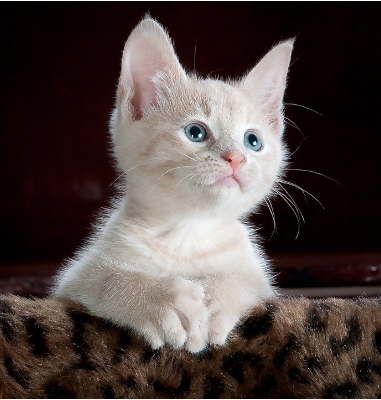
\includegraphics{gatito}

Con la opción \texttt{scale} podemos hacerla más pequeña -o más grande-.
Pero las imágenes en \LaTeX{} no están hechas para insertarse así, sino en una
figura, que es lo que nos permite alterar su alienamiento respecto al texto
y demás propiedades. La siguiente figura está insertada con este código:
\begin{figure}[H] %esta figura es para impedir que se me divida el verbatim
\begin{verbatim}
1   \begin{figure}[H]
2       \centering 
3       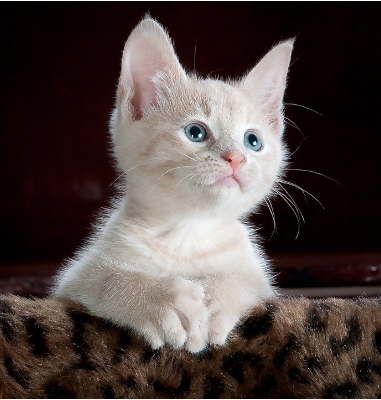
\includegraphics[width=1.0\hsize]{gatito}
4       \caption{Un gato blanco}
5       \label{fig:gatitoBlanco} 
6   \end{figure}
\end{verbatim}
\end{figure}
Vamos a analizar lo que hacen las líneas una a una:
\begin{enumerate}
   \item Crea una figura, que es un cuadro invisible para \LaTeX{}, permite
que lo que haya en ella no se divida y añadirle un título y un símbolo para
referenciarla internamente.
    \begin{itemize}
        \item la opción H (que va entre corchetes) indica a \LaTeX{} que la
        figura debe ir en el sitio en que la hemos escrito en el código, de no
        utilizar esta opción, \LaTeX{} podría decidir un lugar distinto.
    \end{itemize}
    \item Esta línea indica que la figura debe estar centrada.
    \item Esta línea es la que incluye la imagen propiamente dicha.
    \begin{itemize}
        \item La opción (entre corchetes)
            \texttt{width=1.0\textbackslash{}hsize} hace que la imagen ocupe
            el 100 \% del ancho de la página. Si cambias el número ($1.0$) por 
            ejemplo a $0.5$ ocuparía el 50 \%.
        \item Como hemos usado la orden \texttt{graphicspath} en el preámbulo.
        Podemos escribir simplemente el nombre del archivo, sin extensión.
    \end{itemize}
    \item La orden \texttt{caption} pone el título visible que tendrá la figura.
    \item La orden label crea la etiqueta interna de esta figura, y permite 
    luego referenciarla. Esta orden debe ir \textbf{después} de
        \texttt{caption}. Cada tipo de elemento en LaTeX tiene su prefijo, por
        ejemplo, las figuras deben ser \texttt{fig:XXX} y las tablas 
        \texttt{tab:XXX} donde \texttt{XXX} es un nombre arbitrario.
    \item Finalmente, esto termina la figura.
\end{enumerate}

El resultado es el siguiente:
% [H] inserta aquí, t al inicio de la página, b al final... hay muchas opciones
    % Usa "H" si quieres que la figura esté en el mismo orden que como la has
    % escrito, es la opción más intuitiva.
    % (ver sección donde incluyo los paquetes)
% Gracias a que hemos puesto la orden \graphicspath{{./img/}} en el preámbulo
    % de nuestro documento, ahora sólo tenemos que poner el nombre de las
    % imágenes que estén ahí.
%inicio de una figura.
\begin{figure}[H]
    % Centra la imagen
    \centering 
    % Con width=1.0\hsize hacemos que la imagen sea tan ancha como el párrafo,
    % yo lo recomiendo para que las cosas queden alineadas, salvo que por x
    % motivo quieras una imagen más pequeña, entonces cambia 1.0 por otro nº.
    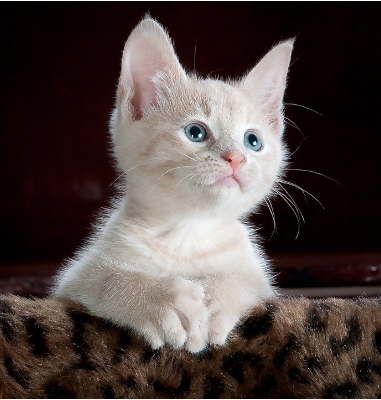
\includegraphics[width=1.0\hsize]{gatito}
    % Título de la figura que se ve
    \caption{Un gato blanco}
    % Etiqueta interna, se usa para referencias la imagen. Esta orden debe ir
    % siempre después de la caption. Cada tipo de figura tiene su formato de 
    % label, por ejemplo las figuras son fig: y las tablas tab:, respétalo o 
    % LaTeX no podrá encontrarlas para los índices.
    \label{fig:gatitoBlanco} 
\end{figure}

Al insertar un párrafo aquí podemos ver cómo se organizan las imágenes, de tal
modo que se insertan en la página necesaria. Las figuras no se dividen a sí
mismas entre páginas.

\begin{figure}[H]
    %centra la imagen (por si no quedaba claro)
    \centering
    % El número antes de hsize es un multiplicador, por ejemplo, podemos hacer
    % que ocupe un tercio de ancho
    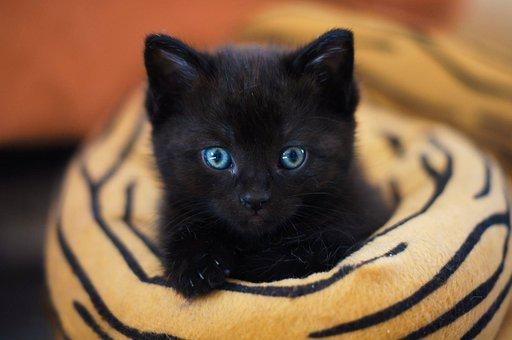
\includegraphics[width=0.3333\hsize]{gatitoNegro}
    \caption{Un gato negro} %caption que se ve
    \label{fig:gatitoNegro} %nombre interno para referenciar luego
\end{figure}

\subsubsection{Referencias cruzadas} \label{subsubsec:referencias cruzadas}
Una referencia cruzada es un punto en el texto en que hablamos de un elemento
del mismo, por ejemplo, si quisiéramos referenciar aquí la figura titulada
<<Un gato negro>>, podríamos ponerlo a mano en el texto: Como se puede ver
en la Figura 2: Un gato negro. Pero, ¿qué pasaría si cambiáramos ese título?
¿Y si incluyéramos una imagen antes de esta y su número cambiara? Tendríamos
que rastrear todas las veces que la hemos mencionado en el documento y cambiarlo
, lo cual sería tedioso y llamaría a errores frecuentes.

Para eso
usaremos el comando \texttt{ref}. Este comando nos permite referenciar una
figura (o cualquier objeto con una etiqueta). 

Si ahora quieres referenciar una figura en un párrafo en \LaTeX{} puedes poner
\texttt{ \textbackslash ref\{nombre de la referencia\}}. Esto insertará el 
número de la figura. Si insertamos \texttt{\textbackslash{}nameref\{nombre
de la referencia\}} aparecerá el título de la misma (la \textit{caption}).

Por ejemplo: como podemos ver en la Figura \ref{fig:gatitoNegro}:
\nameref{fig:gatitoNegro}. A continuación, vamos a insertar una tabla.

\begin{verbatim}
1   \begin{table}[H]
2       \centering
3       \begin{tabular}{|c|r|c|r|}
4           \hline
5           Concepto & Precio Unitario & Cantidad & Subtotal\\ \hline
6           Placa base & \EUR{89,99} & 1 & \EUR{89,99}\\ \hline
7           RAM 8GB DDR4 3200 MHz & \EUR{40,44} & 4 & \EUR{161,76} \\ \hline
8           \textbf{Total}&&&\textbf{\EUR{251,75}} \\ \hline
9       \end{tabular}
10  \caption{Gastos de la reparación}
11  \label{tab:gastos}
12  \end{table}
\end{verbatim}

\begin{enumerate}
\item Inicia la <<figura tabla>>, esto es equivalente a cuando incrustamos
una figura que va a contener una imagen.
\item Hace que la tabla esté centrada, aclaración: cuando la tabla es más 
grande que el tamaño del texto se alinea a la izquierda y se desborda por la
derecha.
\item Empieza la tabla en sí misma, la segunda parte \texttt{\{|c|r|c|r|\}}
indica el número de celdas (que se corresponde con el número de letras) y las 
líneas verticales (|) indican que queremos una línea entre esas dos columnas.
Las líneas verticales son opcionales, pero los especificadores de alineación
deben aparecer en el mismo número que columnas queramos que tenga la tabla.
\item Dibuja una línea horizontal en toda la tabla
\item Es una fila de la tabla, el texto irá en la misma celda hasta que haya
un \textit{et} (\&), así se pasa de columna. Cuando se haya terminado la fila,
se deben poner dos líneas inclinadas invertidas 
(\textbackslash{}\textbackslash{}). 
\item Siguiente fila, apréciese el uso de la orden 
\texttt{\textbackslash{}EUR\{\}}. (ver: \textbf{\ref{ecuaciones}})
\item La siguiente fila.
\item La última fila, nótese que se pueden poner celdas vacías poniendo
dos \emph{et} (\&\&) Y que debe terminarse con \textbackslash{}\textbackslash{}.
\item Termina la tabla
\item Indica el título visible de la tabla.
\item Etiqueta para referencias.
\end{enumerate}
% Esto no sirve para hacer la tabla en sí misma, sino para ponerle captions y
% esas cosas. Es equivalente a \begin{figure} que no inserta una imagen, pero
% nos prepara las cosas para que se comporte como una figura, así podemos
% ponerle título y referenciarla.
\begin{table}[H]
    \centering
    % Aquí defines la tabla en sí misma, tienes que poner tantas letras como
    % columnas vaya a tener la tabla, y puedes poner líneas verticales entre
    % ellas escribiendo este símbolo entre las letras. Estas letras son los
    % especificadores de alineación. Si pones l, la columna se alinea a la
    % izquierda, si pones c, al centro, y si pones r, a la derecha.
    \begin{tabular}{|c|r|c|r|}
    % Esta orden genera una línea entre filas de la tabla.
    \hline
    % En las tablas las celdas se separan con & y las filas con \\
    % Puede haber celdas vacías, pero todas las filas deben tener las mismas
    % celdas.
    Concepto & Precio Unitario & Cantidad & Subtotal\\ \hline
    Placa base & \EUR{89,99} & 1 & \EUR{89,99}\\ \hline
    RAM 8GB DDR4 3200 MHz & \EUR{40,44} & 4 & \EUR{161,76} \\ \hline
    % Aquí podemos ver que hemos puedo celdas vacías. (dos & seguidos)
    \textbf{Total}&&&\textbf{\EUR{251,75}} \\ \hline
\end{tabular}
    % De nuevo, el título que se ve
    \caption{Gastos de la reparación}
    % La referencia interna. 
    \label{tab:gastos}
\end{table}

De nuevo, podemos referenciar el número de la tabla con 
\texttt{\textbackslash ref\{tab:gastos\}} y su
títulos con \nameref{tab:gastos}. \textbf{Nota sobre compilar 
referencias cruzadas:}
 a veces salen signos de
interrogación en lugar de las referencias, no te preocupes, \LaTeX{} a 
veces necesita dos compilaciones para crear la base de datos de referencias.
En el makefile proporcionado ya se compila dos veces, pero si no lo utilizas,
simplemente llama al comando dos veces seguidas.

\subsubsection{Utilización alternativa de las figuras}
Una de las ventajas de utilizar figuras es que el contenido de las mismas no se
divide entre páginas, así que si quisiéramos que una lista en concreto no se
dividiera, podríamos incluirla en un bloque de figura, esta lista, por ejemplo:
\begin{figure}[H]
\begin{itemize}
   \item a
   \item b
   \item c
   \item d
   \item e
   \item f
   \item g
   \item h
   \item i
   \item j
   \item l
   \item m
   \item n
   \item ñ
   \item o
   \item p
   \item q
   \item r
   \item s
   \item t
   \item u
   \item v
   \item w
   \item x
   \item y
   \item z
\end{itemize}
\end{figure}
Esto debe usarse con cuidado, empero, pues generaría muchos espacios en blanco
en nuestro documento.
\subsection{Bibliografía; referencias bibliográficas}
Además de referenciar otras partes de nuestro propio documento (ver
\textbf{\ref{subsubsec:referencias cruzadas}}) es común necesitar una lista
de referencias bibliográficas externas, para esto utilizaremos el paquete
BibTex, que nos permite añadir archivos de bibliografía donde incluiremos
todas las fuentes que necesitemos (podemos incluirlas en distintos archivos
si queremos, e incluir varios), después, nos permitirá citar en el texto esas
fuentes e insertar la sección de bibliografía.

Para crear bibliografía, hay que crear un fichero de extensión .bib, que
contendrá las citas bibliográficas que sean necesarias en un formato especial.
Por ejemplo, en este repositorio hay un directorio llamado bibliography, dentro
del cual hay un archivo llamado sources.bib. Este archivo contiene una fuente
bibliográfica para un libro titulado \emph{El Lenguaje de programación C++}
escrito por Bjarne Stroustrup. El contenido del archivo .bib es el siguiente:
\begin{verbatim}
@book{cpppl,
author = {Stroustrup, Bjarne},
title = {The C++ Programming Language},
year = {2013},
isbn = {0321563840},
publisher = {Addison-Wesley Professional},
edition = {4th},
abstract = {<Resumen del libro, omitido porque es muy largo>}
}
\end{verbatim}

Es decir, para crear un recurso bibliográfico se debe poner una arroba <<@>>,
el tipo de recurso (libro, artículo...), se abre una llave, se pone una 
\textbf{etiqueta}, que es el primer texto: \texttt{cpppl}. Esta es la etiqueta
que usaremos para citar el recurso en el texto.

Hay varios tipos predeterminados de documentos en el paquete biblatex que nos 
permiten citar automáticamente, algunos de ellos son: article, book, thesis,
masterthesis... Pero la principal ventaja del formato bibtex es que muchísimas
plataformas de acceso online permiten copiar directamente el texto que debes
incluir en tu archivo .bib. Más información sobre esto más adelante.

Para citar el libro, utilizaremos el comando
\texttt{\textbackslash cite\{<etiqueta de la fuente>\}}. Veamos un ejemplo, el
código siguiente:
\begin{verbatim}
<<El lenguaje C++ es un superconjunto del lenguaje C>> (\cite[p.~101]{cpppl})
\end{verbatim}
genera este párrafo:

<<El lenguaje C++ es un superconjunto del lenguaje C>> (\cite[p.~101]{cpppl})
Nótese que los paréntesis se han de añadir aparte, y que entre el p. y el
número de página ha de haber una tilde (\~{}), para añadir un espacio. El estilo
de la cita viene dado por las opciones del paquete bibtex incluido en el 
preámbulo, en este caso se ha elegido el estilo de citación APA. Algunos
de los estilos permitidos son:
\begin{table}[H]
\centering
\begin{tabular}{|c|c|}
\hline
    \textbf{Estilo} & \textbf{Argumento} \\ \hline 
    ACS & chem-acs\\\hline
    AIP & phys\\\hline
    Nature& nature\\\hline
    Science & science\\\hline
    IEEE & iee\\\hline
    Chicago& chicago-authordate\\\hline
    MLA & mla\\\hline
    APA & apa\\\hline
\end{tabular}
\caption{Estilo de citación permitidos por el paquete biblatex}
\label{tab:biblatexStyles}
\end{table}
Para elegir estos estilos, debe irse a la línea del preámbulo donde hayamos
incluido el paquete biblatex (recordemos, con la orden usepackage) y modificar
los argumentos de las opciones \texttt{style} y \texttt{citestyle}. Por 
ejemplo, la línea actual es la siguiente:

\begin{verbatim}
\usepackage[backend=biber, style=apa, citestyle=apa]{biblatex}
\end{verbatim}
Si quisiéramos cambiar el estilo para ajustarse al del IEEE, se cambiaría a:
\begin{verbatim}
\usepackage[backend=biber, style=ieee, citestyle=ieee]{biblatex}
\end{verbatim}

Además de citar, necesitaremos imprimir nuestra bibliografía completa en
nuestro documento, para ello, usaremos el comando \texttt{\textbackslash 
printbibliography}. Este comando inserta un título predeterminado que, en 
español (recordemos, paquete babel spanish) es <<Referencias>>, que, además,
no sale en la tabla de contenido. Si queremos omitirlo, podemos añadir la opción
\texttt{heading=none} en la orden, es decir:

\begin{verbatim}
\printbibliography[heading=none]
\end{verbatim}
e incluir nosotros un título de la jerarquía que deseemos justo antes del 
comando. Esto es lo que se ha hecho en este documento. 

Por otro lado, algunas organizaciones exigen que las citas bibliográficas se 
incluyan en notas al pie allí donde se citen. Por suerte \LaTeX{} permite 
crear notas al pie de manera sencilla, simplemente se utiliza el comando
\texttt{\textbackslash footnote\{\}}. Veamos un ejemplo.

\begin{verbatim}
Al final de esta frase va a haber una nota al pie \footnote{Esta es la nota
al pie.}.
\end{verbatim}
genera el siguiente párrafo y su nota el pie correspondiente:

Al final de esta frase va a haber una nota al pie \footnote{Esta es la nota
al pie.}.

Si queremos que en la nota el pie aparezca la cita, simplemente incluimos dentro
del comando \texttt{footnote} el comando \texttt{cite}. Además, tenemos la
opción de incluir en el texto la cita completa (tal y como aparecería en la
bibliografía, con el comando \texttt{\textbackslash fullcite}. Veamos un ejemplo
de una nota el pie con el texto completo de la cita; este código:
\begin{verbatim}
La metaprogramación es una de las características más importantes del lenguaje
C++ \footnote{\fullcite{cpppl}}.
\end{verbatim}
generaría:

La metaprogramación es una de las características más importantes del lenguaje
C++ \footnote{\fullcite{cpppl}}.

\subsubsection{Importar referencias en formato Bibtex}
Como se ha dicho en la sección anterior, muchos servicios permiten importar las
citas bibliográficas directamente en el formato bibtex.
Por ejemplo, busquemos el libro \emph{Historia de la
decadencia y caída del Imperio Romano} en Google Scholar, lo encontramos en
este \href{https://books.google.es/books?id=uydf0KUHpeoC}{enlace}.

Justo al final de esa página hay un botón que nos permite exportar la cita
bibliográfica a varios formatos:

\begin{figure}[H]
    \centering
    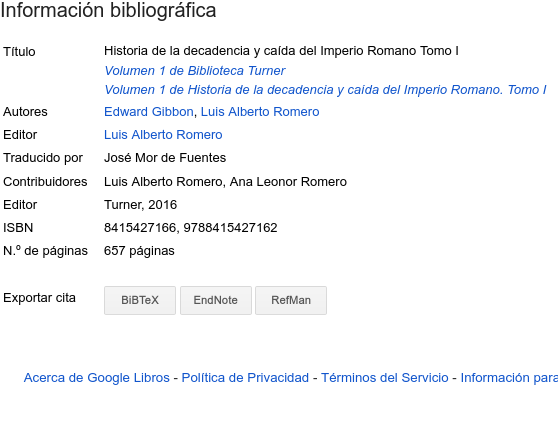
\includegraphics[width=0.75\hsize]{exportarBibtex}
    \caption{Ejemplo de exportar desde Google Books}
    \label{fig:exportGoogle}
\end{figure}

Si elejimos el formato bibtex, nos descargará un archivo con la referencia
que necesitamos, esto nos permitirá copiar su contenido a nuestro archivo
de bibliografía (en este caso, sources.bib). Aunque es recomendable guardar
el archivo descargado aparte por si queremos utilizarlo en otros documentos
a modo de biblioteca personal de citas, en algún lugar de nuestro sistema.

Ahora lo podemos citar:

<<El imperio romano cayó, en parte, por...>> (\cite{gibbon2016historia})

Y se añadirá a nuestra colección de cita en la sección de bibliografía. Bibtex
tiene la ventaja de que aunque en nuestras fuentes bibliográficas haya fuentes
que no hemos citado, no va a incluirlas hasta que las citemos.

\textbf{Nota sobre el formato}: Algunos servicios de documentación, como
el propio Google Books, eliminan los caracteres especiales de sus citas
exportadas (las tildes, la eñe...) y los ponen por ejemplo: 
\texttt{\{\textbackslash\'{}i\}}
en vez de: í. Esto provoca errores, así que simplemente debe cambiarse por
el carácter correspondiente. Otras permiten elegir la codificación, tal
y como está configurado este documento, debe elegirse UTF8. Y debe revisarse
que las etiquetas no contengan estos caracteres especiales de ningún modo, lo
ideal sería sustituirlos por sus equivalentes sin acentos, u por ü, i por í,
etc.

\textbf{Nota sobre la compilación}: Debido a cómo funciona el motor bibtex, 
para que las referencias bibliográficas se creen de manera adecuada, primero
debe compilarse con \texttt{pdflatex}, después, llamar a comando \texttt{biber}
sobre el archivo y después compilar dos veces. En el makefile proporcionado
esto ya se ha hecho, además, utilizando opciones de estos comandos para
que los archivos auxiliares se creen en la carpeta build.

\textbf{Nota para los usuarios de TexStudio}: En este programa, para generar
las fuentes bibliográficas, se debe acudir al menú:
\texttt{Herramientas$\rightarrow$Órdenes$\rightarrow$Biber}
para que se genere la bibliografía, y se debe hacer \textbf{después} de 
compilar una primera vez.

\newpage\section{Decoración e indización}
De momento no se han visto órdenes para crear índices, tablas de contenido,
pies de página y encabezados ni portadas como las que tiene este documento.
En esta sección veremos cómo se ha formateado este documento,
pero lo recomendable es que se quiere copiar alguna característica, simplemente
se incluya el código en tus propios documentos.
\subsection{La portada}
La clase article se creó para artículos científicos, así que no está preparada
para crear portadas tal y como las crean otros editores de texto como 
Word. Lo cual no es un gran inconveniente. Para crear la portada de este
documento se han seguido estos pasos:
\begin{enumerate}
    \item En el preámbulo del documento
    \begin{enumerate}
        \item Se ha usado el comando \texttt{\textbackslash{title}}
        para indicar qué título ha de salir en la portada.
        \item Se ha usado el comando \texttt{\textbackslash{author}}
         para decir qué autor.
    \end{enumerate}
    \item En el contenido del documento
    \begin{enumerate}
        \item Se ha usado el comando \texttt{\textbackslash{maketile}}
        para crear la portada propiamente dicha.
    \end{enumerate}
\end{enumerate}

En términos mínimos, en el documento .tex habrá ahora lo siguiente:
\begin{verbatim}
\documentclass{article}
\title{Título}
\author{Autor de Ejemplo}
\begin{document}
\maketitle
Primer texto del documento.
\end{document}
\end{verbatim}

Esto generará un documento con un título, el nombre del autor y la fecha,
pero el primer texto del documento saldrá en la misma página, y esa página
estará numerada, como 1. Además, la fecha estará en inglés. No es lo ideal.
Las siguientes tareas que llevaremos a cabo son:
\begin{enumerate}
\item Que la portada no se numere.
\item Que la portada esté en su propia página.
\item Modificar la fecha para que salga en español.
\end{enumerate}

Para conseguir la primera tarea, usaremos el comando 
\texttt{\textbackslash{pagenumbering\{gobble\}}}, que hace que las páginas
no se numeren. Este efecto dura hasta que se use otra orden que sobreescriba
este comportamiento.
Para la segunda, vamos a utilizar
el comando \texttt{newpage}, que hace que el siguiente texto salga en la página
siguiente. Ahora, para que las siguiente páginas sí se numeren, usaremos la
orden \texttt{\textbackslash{pagenumbering\{arabic\}}},
así se numerarán con números arábigos.
Finalmente, para la tercera, vamos a utilizar el paquete babel, este
paquete <<traduce>> los textos automáticos (títulos, fechas...) a español,
y da mejor soporte a símbolos del español. En el preámbulo del documento
pondremos simplemente: \texttt{\textbackslash{usepackage\{babel\}}}.
El contenido del documento debería ser, por tanto:
\begin{figure}[H]
\begin{verbatim}
\documentclass{article}

\title{Título}
\author{Autor de Ejemplo}

\usepackage[spanish]{babel}

\begin{document}
\maketitle
\pagenumbering{gobble}
\newpage
\pagenumbering{arabic}

Primer texto del documento.

\end{document}
\end{verbatim}
\end{figure}
Como colofón final, se puede hacer el texto del título y el autor más grande
utilizando los modificadores de tamaño del texto
(ver Tabla \ref{tab:comLetSize}: \nameref{tab:comLetSize}).

\subsection{Tablas de contenido}
Para insertar una tabla de contenido, simplemente se puede incluir en el 
contenido del documento, después de la portada (y de la orden
\texttt{newpage}, la orden
\texttt{\textbackslash{tableofcontents}}, si se desea que el siguiente
texto después de la tabla aparezca en otra página, se puede volver a usar
\texttt{newpage}. Recuerda incluir alguna sección para que el índice no esté
vacío, por ejemplo, incluiremos la sección <<prueba>>. Con estos cambios,
el documento quedaría así:

\begin{figure}[H]
\begin{verbatim}
\documentclass{article}
\title{Título}
\author{Autor de Ejemplo}
\usepackage[spanish]{babel}
\begin{document}
\maketitle
\pagenumbering{gobble}
\newpage
\pagenumbering{arabic}
\tableofcontents
\newpage
\section{Prueba}
Primer texto del documento.
\end{document}
\end{verbatim}
\end{figure}

Para los índices de figuras y tablas, existen las órdenes \texttt{listoffigures}
y \texttt{listoftables}. Recuerda añadir la orden \texttt{newpage} donde
quieras que el texto salga en la página siguiente. El único problema es que,
predeterminadamente, el paquete babel traduce <<tabla>> como <<cuadro>>, de tal
modo que el título de nuestro índice de tablas es <<Índice de cuadros>>, para
arreglar eso se debe añadir una opción al paquete babel, dejando la línea 
donde se incluye como:
\begin{verbatim}
\usepackage[spanish,es-tabla]{babel}
\end{verbatim}
\subsection{Numeración de páginas}
En algunas organizaciones o estilos, se recomienda que el índice -o índices-,
prólogos, prefacios y demás contenido anterior al \textbf{cuerpo} del texto
estén en páginas numeradas en números romanos y el resto en números arábigos.
Vale la pena mencionar que, en español, se desaconseja utilizar números romanos
en minúscula(\cite{raeRoman}). El resto de páginas (las del contenido del
texto), se numeran en números arábigos. Además, personalmente recomiendo, al
menos en el cuerpo del texto, incluir el número total de páginas. Esto es una
medida de integridad, así, en caso de transmisión o impresión del texto, si
alguna página del final se extraviare, el lector se daría cuenta de que faltan.

En general, hay que modificar los encabezados y pies de página. Para esto,
utilizaremos el paquete \texttt{fancyhdr}, que nos permite editar el contenido
en tres posiciones del encabezado y del pie de página: izquierda, central y 
derecha.

Para hacer esto, se deben poner las siguientes órdenes, estas órdenes pueden
ir en el preámbulo del documento o en el contenido. Si se ponen en el contenido
debe tener en cuenta que sólo afectarán a las páginas posteriores a su situación
en el código, es una buena manera de definir numeraciones distintas en distintas
partes del documento como, de hecho, se ha hecho en este.

\Huge{Terminar}\normalsize
\newpage
\section{Licencias y agradecimiento}
Todas las páginas citadas son de sus respectivos creadores, yo sólo me limito
a recopilar sus soluciones o información en un mismo documento. Todas las
imágenes utilizadas son de licencia libre, ver:
\href{https://pixabay.com/service/faq/}{FAQ de Pixabay} o de creación propia.
\newpage
\section{Bibliografía}
\printbibliography[heading=none]
\end{document}
